\documentclass{standalone}
\usepackage{tikz}
\usetikzlibrary{patterns, positioning}
\usepackage[sfdefault]{ClearSans} %% option 'sfdefault' activates Clear Sans as the default text font
\usepackage[T1]{fontenc}

\begin{document}
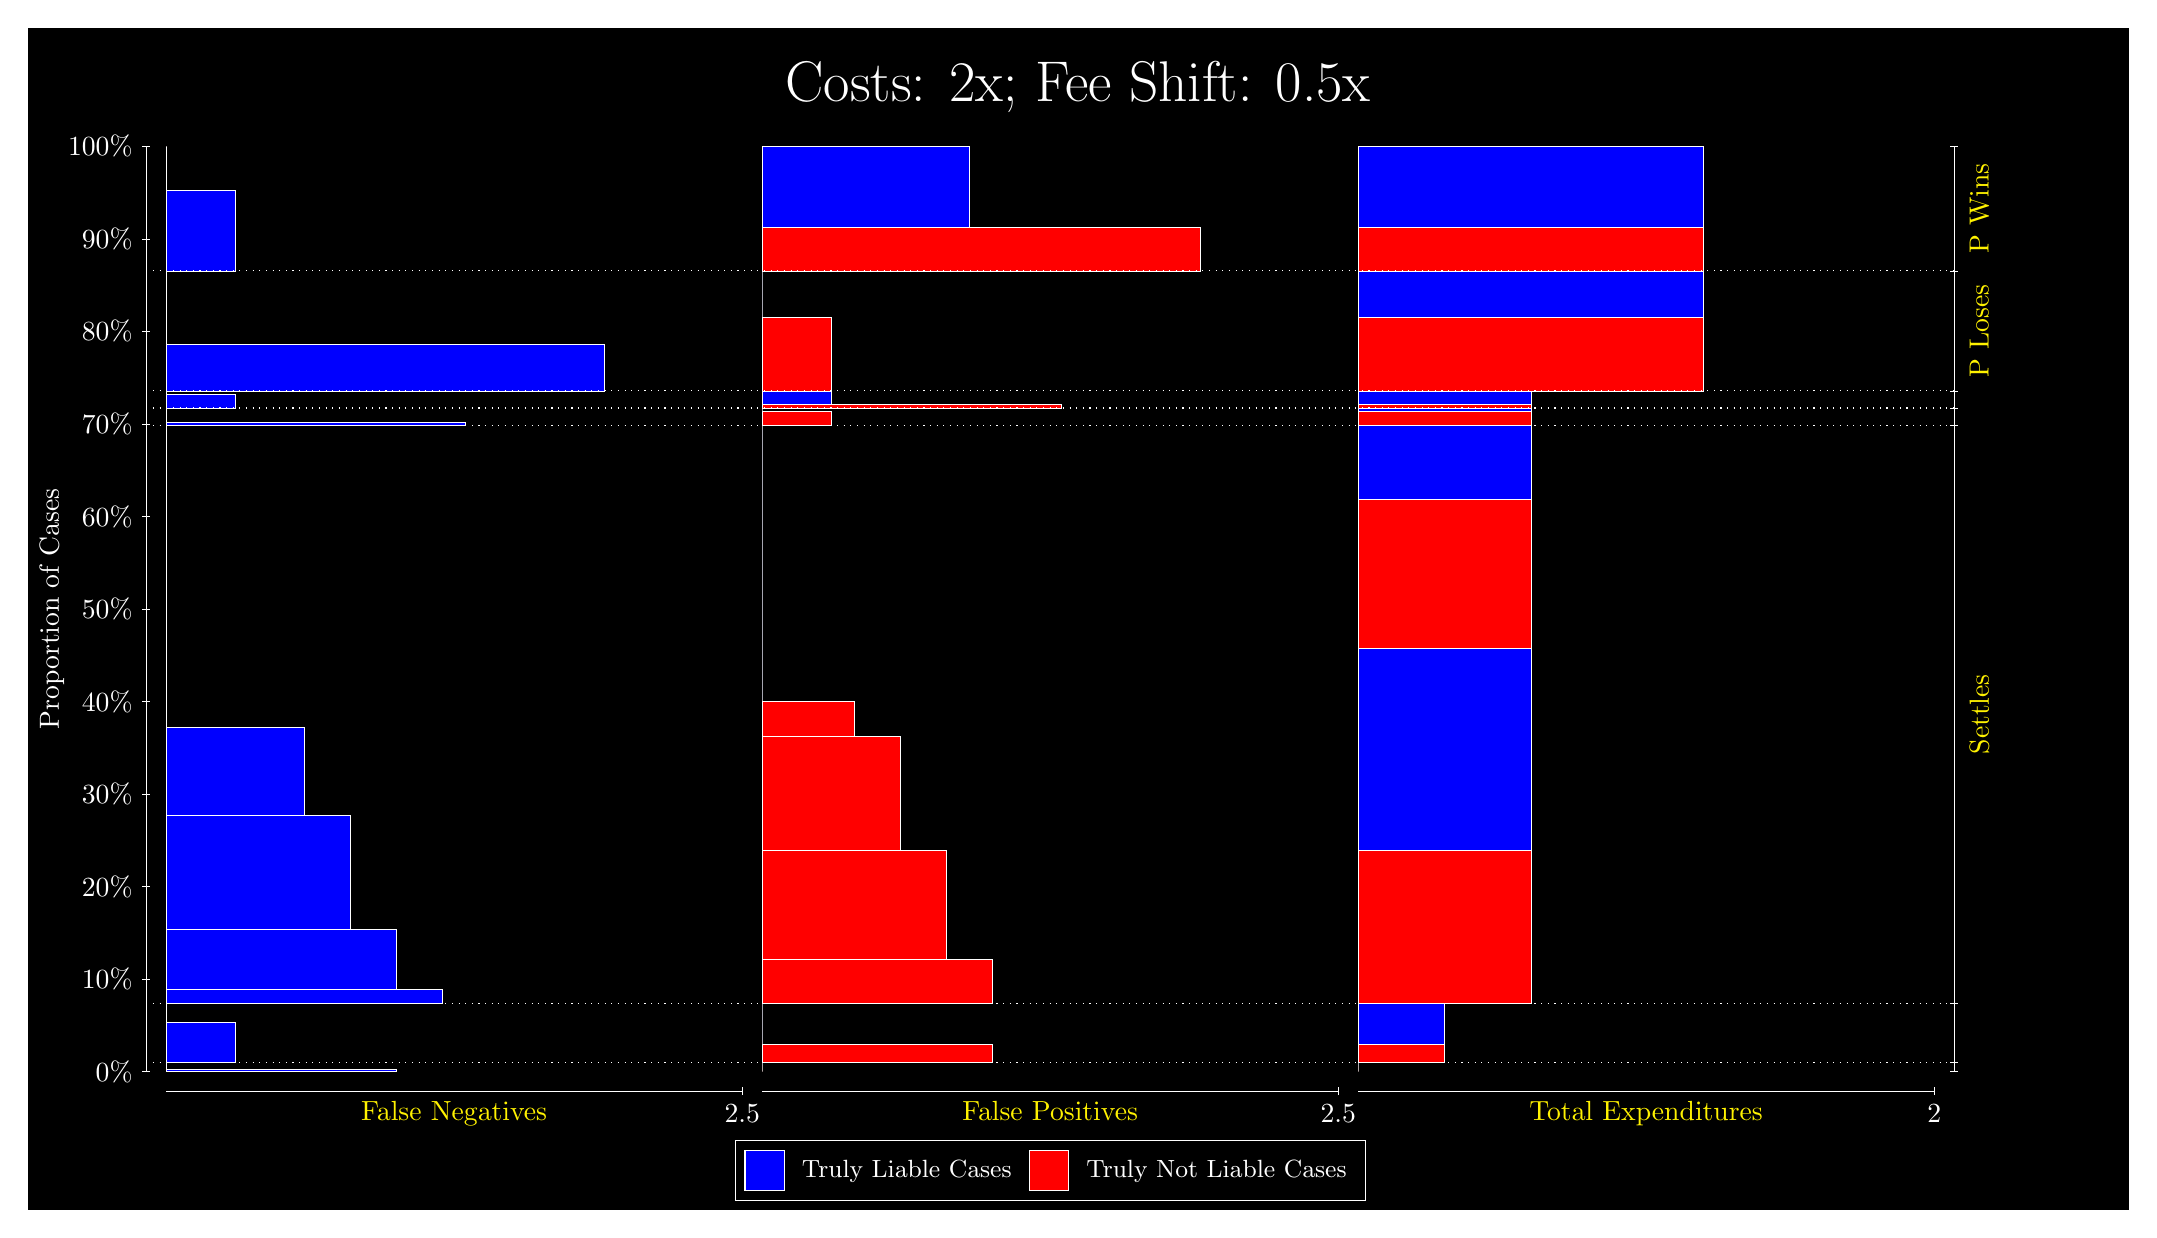
\begin{tikzpicture}
\draw[fill=black] (0,0) rectangle (26.667,15);
\draw[text=white] (0,13.5) rectangle (26.667,15) node[midway] {\huge Costs: 2x; Fee Shift: 0.5x};
\draw[white, very thin] (1.5,1.75) -- (1.5,13.5);
\node[rotate=90, text=white, anchor=center] at (0.3, 7.625) {Proportion of Cases};
\draw[white, very thin] (1.45,1.75) -- (1.55,1.75);
\node[text=white, anchor=east] at (1.45, 1.75) {0\%};
\draw[white, very thin] (1.45,2.925) -- (1.55,2.925);
\node[text=white, anchor=east] at (1.45, 2.925) {10\%};
\draw[white, very thin] (1.45,4.1) -- (1.55,4.1);
\node[text=white, anchor=east] at (1.45, 4.1) {20\%};
\draw[white, very thin] (1.45,5.275) -- (1.55,5.275);
\node[text=white, anchor=east] at (1.45, 5.275) {30\%};
\draw[white, very thin] (1.45,6.45) -- (1.55,6.45);
\node[text=white, anchor=east] at (1.45, 6.45) {40\%};
\draw[white, very thin] (1.45,7.625) -- (1.55,7.625);
\node[text=white, anchor=east] at (1.45, 7.625) {50\%};
\draw[white, very thin] (1.45,8.8) -- (1.55,8.8);
\node[text=white, anchor=east] at (1.45, 8.8) {60\%};
\draw[white, very thin] (1.45,9.975) -- (1.55,9.975);
\node[text=white, anchor=east] at (1.45, 9.975) {70\%};
\draw[white, very thin] (1.45,11.15) -- (1.55,11.15);
\node[text=white, anchor=east] at (1.45, 11.15) {80\%};
\draw[white, very thin] (1.45,12.325) -- (1.55,12.325);
\node[text=white, anchor=east] at (1.45, 12.325) {90\%};
\draw[white, very thin] (1.45,13.5) -- (1.55,13.5);
\node[text=white, anchor=east] at (1.45, 13.5) {100\%};

\draw[white, very thin] (24.457,1.75) -- (24.457,13.5);
\draw[white, very thin] (24.407,1.75) -- (24.507,1.75);
\node[anchor=west] at (24.407, 1.75) {};
\draw[white, very thin] (24.407,1.864) -- (24.507,1.864);
\node[anchor=west] at (24.407, 1.864) {};
\draw[white, very thin] (24.407,2.6165) -- (24.507,2.6165);
\node[anchor=west] at (24.407, 2.6165) {};
\draw[white, very thin] (24.407,9.9582) -- (24.507,9.9582);
\node[anchor=west] at (24.407, 9.9582) {};
\draw[white, very thin] (24.407,10.177) -- (24.507,10.177);
\node[anchor=west] at (24.407, 10.177) {};
\draw[white, very thin] (24.407,10.395) -- (24.507,10.395);
\node[anchor=west] at (24.407, 10.395) {};
\draw[white, very thin] (24.407,11.919) -- (24.507,11.919);
\node[anchor=west] at (24.407, 11.919) {};
\draw[white, very thin] (24.407,13.5) -- (24.507,13.5);
\node[anchor=west] at (24.407, 13.5) {};

\draw[white, very thin, fill=blue] (1.75,1.75) rectangle (4.6775,1.7813);
\draw[white, very thin, fill=red] (1.75,1.7813) rectangle (1.75,1.864);
\draw[white, very thin, fill=blue] (1.75,1.864) rectangle (2.6283,2.3809);
\draw[white, very thin, fill=red] (1.75,2.3809) rectangle (1.75,2.6165);
\draw[white, very thin, fill=blue] (1.75,2.6165) rectangle (5.2631,2.7885);
\draw[white, very thin, fill=blue] (1.75,2.7885) rectangle (4.6775,3.5519);
\draw[white, very thin, fill=blue] (1.75,3.5519) rectangle (4.092,5.0013);
\draw[white, very thin, fill=blue] (1.75,5.0013) rectangle (3.5065,6.1164);
\draw[white, very thin, fill=red] (1.75,6.1164) rectangle (1.75,9.9582);
\draw[white, very thin, fill=blue] (1.75,9.9582) rectangle (5.5558,10.001);
\draw[white, very thin, fill=red] (1.75,10.001) rectangle (1.75,10.177);
\draw[white, very thin, fill=blue] (1.75,10.177) rectangle (2.6283,10.352);
\draw[white, very thin, fill=red] (1.75,10.352) rectangle (1.75,10.395);
\draw[white, very thin, fill=blue] (1.75,10.395) rectangle (7.3123,10.981);
\draw[white, very thin, fill=red] (1.75,10.981) rectangle (1.75,11.919);
\draw[white, very thin, fill=blue] (1.75,11.919) rectangle (2.6283,12.942);
\draw[white, very thin, fill=red] (1.75,12.942) rectangle (1.75,13.5);
\draw[white, very thin, fill=red] (9.3189,1.75) rectangle (9.3189,1.8327);
\draw[white, very thin, fill=blue] (9.3189,1.8327) rectangle (9.3189,1.864);
\draw[white, very thin, fill=red] (9.3189,1.864) rectangle (12.246,2.0995);
\draw[white, very thin, fill=blue] (9.3189,2.0995) rectangle (9.3189,2.6165);
\draw[white, very thin, fill=red] (9.3189,2.6165) rectangle (12.246,3.1803);
\draw[white, very thin, fill=red] (9.3189,3.1803) rectangle (11.661,4.5639);
\draw[white, very thin, fill=red] (9.3189,4.5639) rectangle (11.075,6.0101);
\draw[white, very thin, fill=red] (9.3189,6.0101) rectangle (10.49,6.4583);
\draw[white, very thin, fill=blue] (9.3189,6.4583) rectangle (9.3189,9.9582);
\draw[white, very thin, fill=red] (9.3189,9.9582) rectangle (10.197,10.134);
\draw[white, very thin, fill=blue] (9.3189,10.134) rectangle (9.3189,10.177);
\draw[white, very thin, fill=red] (9.3189,10.177) rectangle (13.125,10.219);
\draw[white, very thin, fill=blue] (9.3189,10.219) rectangle (10.197,10.395);
\draw[white, very thin, fill=red] (9.3189,10.395) rectangle (10.197,11.333);
\draw[white, very thin, fill=blue] (9.3189,11.333) rectangle (9.3189,11.919);
\draw[white, very thin, fill=red] (9.3189,11.919) rectangle (14.881,12.477);
\draw[white, very thin, fill=blue] (9.3189,12.477) rectangle (11.954,13.5);
\draw[white, very thin, fill=red] (16.888,1.75) rectangle (16.888,1.8327);
\draw[white, very thin, fill=blue] (16.888,1.8327) rectangle (16.888,1.864);
\draw[white, very thin, fill=red] (16.888,1.864) rectangle (17.986,2.0995);
\draw[white, very thin, fill=blue] (16.888,2.0995) rectangle (17.986,2.6165);
\draw[white, very thin, fill=red] (16.888,2.6165) rectangle (19.083,4.5639);
\draw[white, very thin, fill=blue] (16.888,4.5639) rectangle (19.083,7.1285);
\draw[white, very thin, fill=red] (16.888,7.1285) rectangle (19.083,9.0228);
\draw[white, very thin, fill=blue] (16.888,9.0228) rectangle (19.083,9.9582);
\draw[white, very thin, fill=red] (16.888,9.9582) rectangle (19.083,10.134);
\draw[white, very thin, fill=blue] (16.888,10.134) rectangle (19.083,10.177);
\draw[white, very thin, fill=red] (16.888,10.177) rectangle (19.083,10.219);
\draw[white, very thin, fill=blue] (16.888,10.219) rectangle (19.083,10.395);
\draw[white, very thin, fill=red] (16.888,10.395) rectangle (21.279,11.333);
\draw[white, very thin, fill=blue] (16.888,11.333) rectangle (21.279,11.919);
\draw[white, very thin, fill=red] (16.888,11.919) rectangle (21.279,12.477);
\draw[white, very thin, fill=blue] (16.888,12.477) rectangle (21.279,13.5);
\draw[white, dotted] (1.5,1.864) -- (24.457,1.864);
\draw[white, dotted] (1.5,2.6165) -- (24.457,2.6165);
\draw[white, dotted] (1.5,9.9582) -- (24.457,9.9582);
\draw[white, dotted] (1.5,10.177) -- (24.457,10.177);
\draw[white, dotted] (1.5,10.395) -- (24.457,10.395);
\draw[white, dotted] (1.5,11.919) -- (24.457,11.919);
\draw[white, very thin] (1.75,1.5) -- (9.0689,1.5);
\node[text=yellow, anchor=north] at (5.4094, 1.5) {False Negatives};
\draw[white, very thin] (9.0689,1.45) -- (9.0689,1.55);
\node[text=white, anchor=north] at (9.0689, 1.45) {2.5};

\draw[white, very thin] (9.3189,1.5) -- (16.638,1.5);
\node[text=yellow, anchor=north] at (12.978, 1.5) {False Positives};
\draw[white, very thin] (16.638,1.45) -- (16.638,1.55);
\node[text=white, anchor=north] at (16.638, 1.45) {2.5};

\draw[white, very thin] (16.888,1.5) -- (24.207,1.5);
\node[text=yellow, anchor=north] at (20.547, 1.5) {Total Expenditures};
\draw[white, very thin] (24.207,1.45) -- (24.207,1.55);
\node[text=white, anchor=north] at (24.207, 1.45) {2};



\node[text=yellow, centered, rotate=90] at (24.777, 6.2873) {Settles};


\node[text=yellow, centered, rotate=90] at (24.777, 11.157) {P Loses};
\node[text=yellow, centered, rotate=90] at (24.777, 12.71) {P Wins};

\draw (12.978300999999998,1.5) node[draw=none] (baseCoordinate) {};
\begin{scope}[align=center]
        \matrix[scale=0.5, draw=white, below=0.5cm of baseCoordinate, nodes={draw}, column sep=0.1cm]{
            \node[rectangle, draw, minimum width=0.5cm, minimum height=0.5cm, fill=blue] {}; &
            \node[draw=none, font=\small, text=white] (B) {Truly Liable Cases}; &
            \node[rectangle, draw, minimum width=0.5cm, minimum height=0.5cm, fill=red] {}; &
            \node[draw=none, font=\small, text=white] (B) {Truly Not Liable Cases}; \\
            };
\end{scope}

\end{tikzpicture}
\end{document}